\documentclass[a4paper,12pt]{article}
\usepackage[utf8]{inputenc}
\usepackage[T1]{fontenc}

\title{E3 Reinforcement learning}
\author{arthur CLEMENT}
% \date{December 2016 \thanks{nasa}}

% \usepackage{natbib}
\usepackage{graphicx}
\usepackage{amsmath}
% \usepackage[backend=biber,style=verbose-trad2]{biblatex}
\usepackage{booktabs}
\usepackage{xcolor}
\usepackage{soul}
\usepackage{sectsty}
\usepackage[french,english]{babel}
\usepackage{listings}
\usepackage{hyperref}
% \usepackage[french,noline,tworuled]{algorithm2e}
\usepackage{fancyhdr}
% \usepackage[nottoc]{tocbibind}
\usepackage{setspace}

\pagestyle{fancy}

\lhead{
\includegraphics[width=3cm]{Microsoft_logo_cropped.png}}
\rhead{
\includegraphics[width=2.5cm]{Simplon_logo.png}}
\setlength{\headheight}{28.6625pt}

\hypersetup{
    colorlinks,
    citecolor=black,
    filecolor=black,
    linkcolor=black,
    urlcolor=black
}

% \definecolor{backgroundgray}{gray}{0.93}

% \sectionfont{\sffamily \color{red} \fontsize{20}{0} \selectfont}
\sectionfont{\color{red} \fontsize{20}{0} \selectfont}
% \subsectionfont{\sffamily \color{green!50!black}  \fontsize{15}{0} \selectfont}
\subsectionfont{\color{green!50!black} \fontsize{15}{0} \selectfont}
\subsubsectionfont{\sffamily \color{blue!40!black}}

\onehalfspacing

\begin{document}

\begin{titlepage}
    \pagenumbering{gobble}
    \thispagestyle{fancy}
	\centering
	
\includegraphics[width=0.65\textwidth]{Ecole_IA_logo_cropped.png}\par
	\vspace{1cm}
% 	\hrulefill\par
% 	{\scshape\LARGE Columbidae University \par}
% 	\vspace{1cm}
% 	{\scshape\Large Final year project\par}
% 	\vspace{1.5cm}
% 	{\huge\bf Pigeons love doves\par}
% 	\vspace{2cm}
% 	{\Large\itshape John Birdwatch\par}
% 	\vfill
% 	supervised by\parhttps://www.overleaf.com/project/62051a2cc210143f88e1de3a
% 	Dr.~Mark \textsc{Brown}

% 	\vfill

    % Bottom of the page
% 	{\large \today}

    \vspace{3cm}
    {\scshape\Large E3 - Cas pratique 2}\par
    \vspace{1cm}
    {\huge\bf Reinforcement learning}\par
    \vfill
    Arthur {\scshape Clément}

\end{titlepage}

\sffamily

\newpage
\pagenumbering{arabic}
\renewcommand*\contentsname{Sommaire}
\tableofcontents

\section{Introduction}

Dans l'industrie moderne, les applications de l'intelligence artificielle (au sens large) sont dominées par l'apprentissage supervisé et non supervisé, où il est nécessaire d'assembler un jeu de données pour que l'algorithme choisi puisse en apprendre les caractéristiques. Le modèle pourra alors, dans le cas de l'apprentissage supervisé, généraliser ses connaissances sur de nouvelles données, ou dans le cas de l'apprentissage non supervisé, organiser les données entre elles de la manière qui lui semblera optimale. Dans tous les cas, les performances de ces modèles sont entièrement dépendantes de la qualité et de la quantité des données d'apprentissage, ce qui nécessite de la part des entreprises qui désirent intégrer l'intelligence artificielle dans leurs activités ou leurs services un travail complexe de collecte, d'analyse, de nettoyage et de traitement d'une base de donnée de volume suffisant pour atteindre leurs objectifs de performance.\par
\medskip
Il existe cependant un domaine de l'intelligence artificielle qui ne nécessite pas la fastidieuse constitution d'une base de donnée: l'apprentissage par renforcement. L'apprentissage par renforcement consiste généralement à produire un agent capable de prendre la meilleure décision possible dans une situation donnée. Pour cela, on simule un environnement dans lequel l'agent va évoluer. L'agent va devoir prendre une séquence de décisions basées sur les différents états de l'environnement dans lequel il se trouve; en retour, l'environnement de l'agent va évoluer et communiquer à l'agent une récompense basée sur l'évolution (la récompense sera positive ou négative en fonction de l'objectif arbitraire que l'on fixe à l'agent). En évoluant ainsi dans son environnement, l'agent va se constituer sa propre base de données {état, décision, récompense} qu'il pourra alors utiliser comme base d'apprentissage.\par

\begin{center}
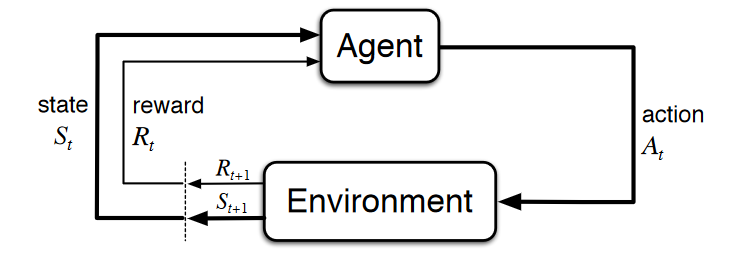
\includegraphics[width=1\textwidth]{E3_images/agent-environment_cropped.png}\par
\end{center}

Comme certains environnements ont un nombre incalculable d'états possibles (jeu de GO, environnements à états continus ...), ou que l'environnement ne peut pas être décrit complètement (poker), les algorithmes avancés d'apprentissage par renforcement utilisent des modèles d'apprentissage profond pour représenter les états et appréhender des états nouveaux de la bonne manière. On se propose ici de présenter l'état de l'art de l'apprentissage par renforcement profond, ainsi que de l'analyse des sources utilisées.\par

\medskip
\section{\'Etat de l'art du domaine}

% \medskip
% \subsection{Jeux ATARI}

\medskip
\subsection{Méthode d'évaluation: "The Arcade Learning Environment"}

\`A cause de la nature des domaines d'application de l'apprentissage par renforcement, il n'existe pas de base de données de référence comme \textbf{ImageNet} \cite{imagenet} ou \textbf{MNIST} \cite{mnist} pour les modèles de vision par ordinateurs. \`A la place, les modèles d'apprentissage par renforcement ont besoin d'environnements de référence pour pouvoir comparer leurs performances. C'est dans ce but qu'à été introduit l'\textbf{ALE} (Arcade Learning Environement) \cite{bellemare13arcade, arcade2} en open-source en 2013, un répertoire de dizaines de jeux de la platefrome ATARI 2600 qui proposent chacun des challenges différents, et qui ont l'avantage de pouvoir être joués par des êtres humains, ce qui permet de comparer facilement les performances des modèles avec les performances humaines.\par

\medskip
\subsection{Deep Q-Network}

Publié par DeepMind en 2013 puis amélioré en 2015, le \textbf{Deep-Q Network} \cite{deep_q_learning, mnih2015humanlevel} est devenu rapidement une référence dans le domaine de l'apprentissage par renforcement, d'une part par son utilisation innovante d'un agent doté d'un réseau de neurones convolutionnel, et d'autre part car ses performances sont proches, voire dépassent celles d'un être humain.\par
\medskip
\begin{center}
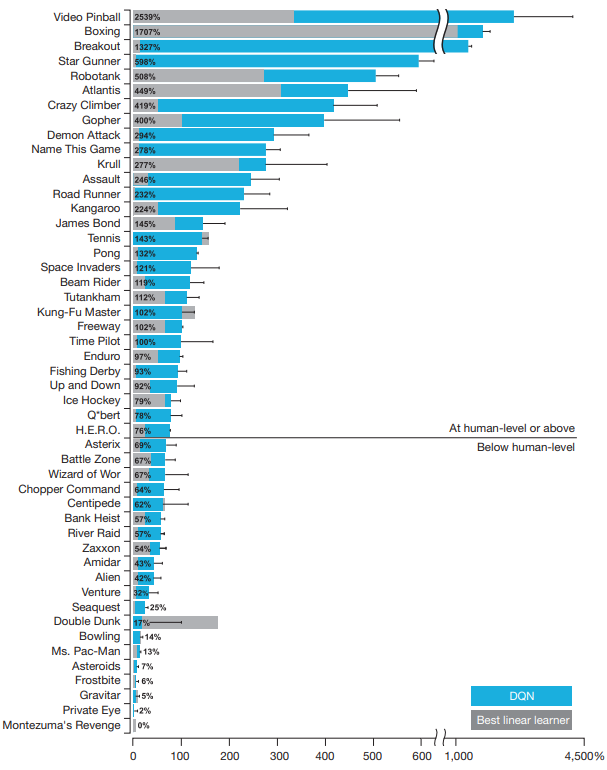
\includegraphics[width=1\textwidth]{E3_images/DQN.png}\par
{\small Performances du Deep Q-Network comparées aux performances humaines (0\% pour des actions aléatoires, 100\% pour un joueur professionel)\par}
\end{center}
\medskip
Pendant l'entraînement,  l'agent va se constituer un base d'expérience, qui associera les pixels de l'écran de jeu, l'action choisie et la récompense obtenue. \'A intervalles réguliers, le modèle sera entraîné sur un échantillon aléatoire d'expériences, et pourra ainsi apprendre quelles actions donneront les meilleures récompense, quelle que soit la situation de l'environnement.\par

\medskip
\subsection{Double Deep Q-Network}

Les travaux qui ont amené le \textbf{Double Deep Q-Network} \cite{double_ddqn} sont basé sur ceux du Deep Q-Network. Après avoir observé que le Deep Q-Network avait tendance à surestimer les récompenses des actions possibles, Les chercheurs de DeepMind ont mis en oeuvre l'idée de découpler la prédiction de la récompense d'une action du choix de l'action à prendre lui-même entre deux modèles, et de n'entraîner que l'un d'entre eux durant l'apprentissage. La stabilité obtenue dans la modélisation interne du modèle permet des performance dépassant celles du Deep Q-Network pour plusieurs jeux ATARI.\par

\medskip
\subsection{R2D2}

Le modèle "\textbf{Recurrent Replay Distributed DQN}" (R2D2) \cite{r2d2} reprend les idées du Deep Q-Network, mais sépare les étapes d'exploration de l'environnement et d'entraînement du modèle sur ces expériences ; il peut ainsi récupérer les expériences de plusieurs modèles explorant l'environnement en parallèle, et ainsi se constituer une base d'experiences plus diverse. Les auteurs du papier déclarent que le modèle atteint un nouvel état de l'art dans le domaine des jeux ATARI, dépassant les précedents records.\par

\medskip
\subsection{MuZero}

\textbf{MuZero} \cite{muzero} pousse encore plus loin le concept d'apprentissage par renforcement basé sur modèle, en produisant un algorithme capable de prédire le résultat de ses actions plusieurs coups à l'avance, en utilisant une méthode de Monte-Carlo tree search. Les performances publiées sur les jeux de la plateforme ATARI definissent un nouvel état de l'art dans le domaine.\par

\medskip
\subsection{Agent57}

Le modèle \textbf{Agent57} \cite{agent57} est le premier qui est parvenu à dépasser les performances humaines sur l'ensembles des 57 jeux ATARI proposé par l'ALE. Il utilise la méthode des agents distribués de R2D2 en incluant une récompense parallèle qui favorise l'exploration intensive. En effet, certains jeux nécessitent des dizaines d'actions correctes avant de parvenir à la moindre récompense ; les modèles qui n'explorent pas assez profondément l'environnement risquent de rater la solution.\par

\medskip
\section{Conclusion}

\medskip
\subsection{Synthèse}

% En ce qui concerne l'apprentissage par renforcement,
Les solutions présentées ici ne sont qu'une présentation des meilleurs résultats jusqu'ici dans le domaine de l'apprentissage par renforcement. Bien que les performances de l'état de l'art ne tendent qu'à évoluer, il semble que ces modèles proposent des solutions fiables types de problèmes posés.\par
\medskip
Compte tenu de la quantité d'options disponibles, et de la diversité des environnements à résoudre, la meilleure solution n'est pas toujours de prendre le modèle plus performant selon les métriques des jeux ATARI ; mais c'est la base la plus fiable disponible.

\medskip
\subsection{Analyse des sources}

Chaque solution est issue d'un papier de recherche scientifique peer-reviewed, la majorité d'entre eux provenant du site \textit{paperswithcode.com}, reconnu pour sa fiabilité dans le domaine du machine learning.

% unsrt, plain
\medskip
\bibliographystyle{unsrt}
\bibliography{refs_E3}
\end{document}
